%!TEX root = ../template.tex
%%%%%%%%%%%%%%%%%%%%%%%%%%%%%%%%%%%%%%%%%%%%%%%%%%%%%%%%%%%%%%%%%%%%
%% chapter3.tex
%% NOVA thesis document file
%%
%% Chapter with a short latex tutorial and examples
%%%%%%%%%%%%%%%%%%%%%%%%%%%%%%%%%%%%%%%%%%%%%%%%%%%%%%%%%%%%%%%%%%%%

\typeout{NT FILE chapter3.tex}%

\makeatletter
\newcommand{\ntifpkgloaded}{%
	\@ifpackageloaded%
}
\makeatother

\chapter{Exact Algorithms for the \Gls{TSP}} \label{chapt:3}

This chapter provides an in-depth examination of exact algorithms for solving the \Gls{TSP}, incorporating detailed pseudocode to clarify the operational principles of each method. Through these algorithms, we explore the computational landscape of finding optimal solutions to the \Gls{TSP}.

\section{Overview of Exact Algorithms}

Exact algorithms for the \Gls{TSP} are characterized by their ability to invariably find the optimal solution, albeit with computational costs that can become prohibitive as the number of cities increases. These algorithms serve as a theoretical and practical foundation for understanding the limits of computational resolution of the \Gls{TSP}.

\subsection{Brute-Force Method}

The brute-force method systematically examines every possible tour to identify the one with the shortest total distance. Despite its simplicity, the exponential growth of calculations makes it impractical for non-trivial sizes.

\begin{algorithm}
	\caption{TSP Brute Force}\label{bruteforce}
	\begin{algorithmic}[1]
		\Procedure{BruteForceTSP}{$cities$}
		\State $min\_distance \gets \infty$
		\State $min\_tour \gets \emptyset$
		\ForAll{tours $t$ of $cities$}
		\State $distance \gets$ \textsc{TourDistance}($t$)
		\If{$distance < min\_distance$}
		\State $min\_distance \gets distance$
		\State $min\_tour \gets t$
		\EndIf
		\EndFor
		\State \Return $min\_tour$
		\EndProcedure
	\end{algorithmic}
\end{algorithm}
\begin{figure}[htbp]
	\centering
	\begin{subfigure}[b]{0.45\textwidth}
		\centering
		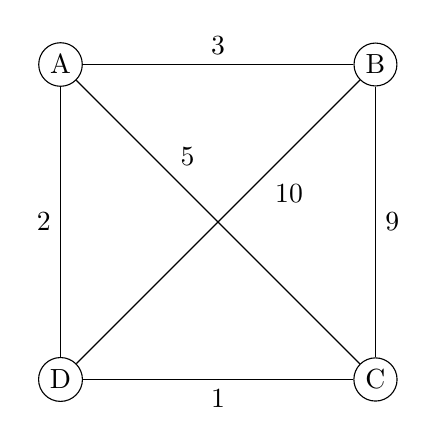
\begin{tikzpicture}
			% Define nodes with their coordinates
			\node[circle, draw=black, text=black, inner sep=2pt] (A) at (-2, 2) {A};
			\node[circle, draw=black, text=black, inner sep=2pt,] (B) at (2, 2) {B};
			\node[circle, draw=black, text=black, inner sep=2pt] (C) at (2, -2) {C};
			\node[circle, draw=black, text=black, inner sep=2pt] (D) at (-2, -2) {D};

			% Draw edges with labels
			\draw (A) -- (B) node[midway, above] {3};
			\draw (A) -- (D) node[midway, left] {2};
			\draw (B) -- (D) node[pos=1/3, below right] {10};
			\draw (B) -- (C) node[midway,  right] {9};
			\draw (D) -- (C) node[midway, below] {1};
			\draw (A) -- (C) node[pos=1/3, above right] {5};

		\end{tikzpicture}
		\caption{Starting graph with four cities}
		\label{fig:subfig1}
	\end{subfigure}
	\hfill
	\begin{subfigure}[b]{0.45\textwidth}
		\centering
		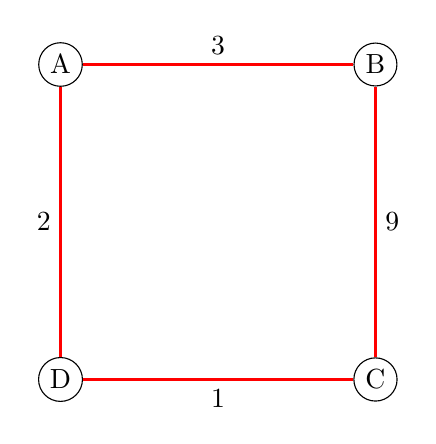
\begin{tikzpicture}
			% Define nodes with their coordinates
			\node[circle, draw=black, text=black, inner sep=2pt] (A) at (-2, 2) {A};
			\node[circle, draw=black, text=black, inner sep=2pt,] (B) at (2, 2) {B};
			\node[circle, draw=black, text=black, inner sep=2pt] (C) at (2, -2) {C};
			\node[circle, draw=black, text=black, inner sep=2pt] (D) at (-2, -2) {D};

			% Draw edges with labels
			\draw (A) -- (B) node[midway, above] {3};
			\draw (A) -- (D) node[midway, left] {2};
			% \draw (B) -- (D) node[pos=1/3, below right] {10};
			\draw (B) -- (C) node[midway,  right] {9};
			\draw (D) -- (C) node[midway, below] {1};
			% \draw (A) -- (C) node[pos=1/3, above right] {5};

			\draw[thick, red] (A) -- (B) -- (C) -- (D) -- (A);

		\end{tikzpicture}
		\caption{Optimal path with total distance 15}
		\label{fig:subfig2}
	\end{subfigure}

	\begin{subfigure}[b]{0.45\textwidth}
		\centering
		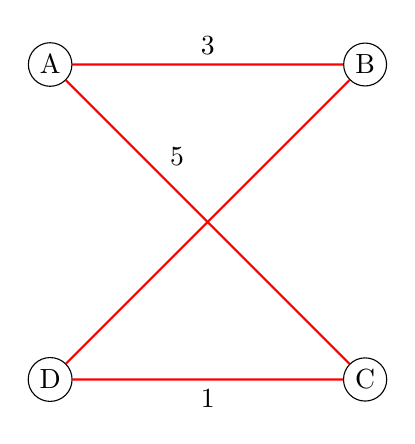
\begin{tikzpicture}
			% Define nodes with their coordinates
			\node[circle, draw=black, text=black, inner sep=2pt] (A) at (-2, 2) {A};
			\node[circle, draw=black, text=black, inner sep=2pt,] (B) at (2, 2) {B};
			\node[circle, draw=black, text=black, inner sep=2pt] (C) at (2, -2) {C};
			\node[circle, draw=black, text=black, inner sep=2pt] (D) at (-2, -2) {D};

			% Draw edges with labels
			\draw (A) -- (B) node[midway, above] {3};
			% \draw (A) -- (D) node[midway, left] {2};
			% \draw (B) -- (D) node[pos=1/3, below right] {10};
			% \draw (B) -- (C) node[midway,  right] {9};
			\draw (D) -- (C) node[midway, below] {1};
			\draw (A) -- (C) node[pos=1/3, above right] {5};

			\draw[thick, red] (A) -- (B) -- (D) -- (C) -- (A);

		\end{tikzpicture}
		\caption{Alternative path with total distance 19}
		\label{fig:subfig3}
	\end{subfigure}
	\hfill
	\begin{subfigure}[b]{0.45\textwidth}
		\centering
		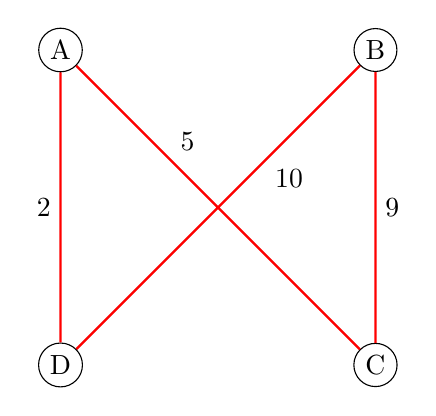
\begin{tikzpicture}
			% Define nodes with their coordinates
			\node[circle, draw=black, text=black, inner sep=2pt] (A) at (-2, 2) {A};
			\node[circle, draw=black, text=black, inner sep=2pt,] (B) at (2, 2) {B};
			\node[circle, draw=black, text=black, inner sep=2pt] (C) at (2, -2) {C};
			\node[circle, draw=black, text=black, inner sep=2pt] (D) at (-2, -2) {D};

			% Draw edges with labels
			% \draw (A) -- (B) node[midway, above] {3};
			\draw (A) -- (D) node[midway, left] {2};
			\draw (B) -- (D) node[pos=1/3, below right] {10};
			\draw (B) -- (C) node[midway,  right] {9};
			% \draw (D) -- (C) node[midway, below] {1};
			\draw (A) -- (C) node[pos=1/3, above right] {5};

			\draw[thick, red] (A) -- (D) -- (B) -- (C) -- (A);

		\end{tikzpicture}
		\caption{Alternative path with total distance 26}
		\label{fig:subfig4}
	\end{subfigure}

	\caption{Brute force TSP with four cities}
	\label{fig:four_subfigures}
\end{figure}

The computational complexity of this method is $O(n!)$, which reflects the factorial number of tours that must be evaluated.

\subsection{Bellman-Held-Karp Algorithm}

The Bellman-Held-Karp algorithm represents a significant advancement in exact solutions for the \Gls{TSP} by exploiting dynamic programming to reduce the computational burden. This approach computes the shortest path by dividing the problem into smaller subproblems and storing the results of these subproblems to avoid redundant calculations exploiting dynamic programming.

\begin{algorithm}
	\caption{Bellman-Held-Karp Algorithm}\label{bellmanheldkarp}
	\begin{algorithmic}[1]
		\Procedure{BellmanHeldKarp}{$cities$}
		\State Create a table $distances$ to store the shortest paths
		\State Initialize all entries in $distances$ to $\infty$
		\State $distances[1][\{1\}] \gets 0$ \Comment{Starting city}
		\For{$m = 2$ to $|cities|$}
		\ForAll{subsets $S$ of $cities$ of size $m$ containing 1}
		\ForAll{$j \in S, j \neq 1$}
		\State $distances[j][S] \gets \min_{k \neq j, k \in S} (distances[k][S\setminus\{j\}] + distance(k, j))$
		\EndFor
		\EndFor
		\EndFor
		\State \Return $\min_{j}(distances[j][cities] + distance(j, 1))$
		\EndProcedure
	\end{algorithmic}
\end{algorithm}

The Bellman-Held-Karp algorithm operates with a time complexity of $O(n^2 \cdot 2^n)$~\ref{fig:agl_complexity}, making it significantly more efficient than the brute-force method for moderate-sized problem instances. However, the exponential component of its complexity still limits its practical applicability to relatively small instances of the \Gls{TSP}.

% \begin{figure}[htbp]
% 	\centering
% 	\begin{tikzpicture}[node distance=2cm]
% 		\node (A) [circle,draw] {A};
% 		\node (B) [circle,draw, right of=A] {B};
% 		\node (C) [circle,draw, below right of=A] {C};
% 		\node (D) [circle,draw, below left of=A] {D};

% 		\draw (A) -- (B) node [midway, above] {5};
% 		\draw (A) -- (C) node [midway, right] {4};
% 		\draw (A) -- (D) node [midway, left] {6};
% 		\draw (B) -- (C) node [midway, right] {3};
% 		\draw (B) -- (D) node [midway, above] {7};
% 		\draw (C) -- (D) node [midway, below] {2};

% 		\node [below=1cm of C] {Sottoproblema: Cammino minimo da A a D passando per B e C};
% 	\end{tikzpicture}
% 	\caption{Visualizzazione di un sottoproblema nella programmazione dinamica per il TSP}
% 	\label{fig:dynamic-programming-subproblem}
% \end{figure}

\subsubsection{Branch and Bound}

Branch and Bound (\Gls{BnB}) is a general algorithmic technique that can be applied to various combinatorial optimization problems, including the \Gls{TSP}. It systematically explores the solution space by dividing it into smaller subsets (branching) and using bounds to eliminate subsets that do not contain the optimal solution, thus reducing the search space.

\begin{algorithm}
	\caption{\Gls{BnB} for the \Gls{TSP}}\label{branchbound}
	\begin{algorithmic}[1]
		\Procedure{BranchAndBoundTSP}{$cities$}
		\State Initialize a priority queue $Q$ with a partial solution starting from the first city
		\State $min\_distance \gets \infty$
		\While{$Q$ is not empty}
		\State Take the partial solution with the lowest lower bound from $Q$
		\If{it represents a complete tour}
		\If{its cost is less than $min\_distance$}
		\State Update $min\_distance$ and record the tour
		\EndIf
		\Else
		\State Branch by adding a city to the partial solution
		\State Calculate bounds for the new partial solutions
		\State Add the new partial solutions to $Q$
		\EndIf
		\EndWhile
		\State \Return $min\_distance$
		\EndProcedure
	\end{algorithmic}
\end{algorithm}

The efficiency of \Gls{BnB} for the \Gls{TSP} depends significantly on the bounding function used to estimate the lower bound of partial solutions. An effective bound can lead to substantial reductions in the search space, allowing the algorithm to find the optimal solution more quickly than exhaustive search methods. However, its worst-case time complexity remains $O(n!)$~\ref{fig:agl_complexity}, which means that for very large problem instances, even this sophisticated approach may not be practical.

\section{Analysis of Exact Algorithms}

\subsection{Computational Feasibility}

Exact algorithms for the \Gls{TSP}, such as the brute-force method, dynamic programming, and the Bellman-Held-Karp algorithm, offer theoretical guarantees for finding the optimal tour. However, their computational feasibility is significantly compromised as the number of cities increases. The factorial growth rate of the brute-force method's complexity and the exponential growth rate of the Bellman-Held-Karp complexity limit their practical application to relatively small instances of the \Gls{TSP}.

\begin{center}
	\begin{figure}[h]
		\centering
		\caption{Complexity of Exact Algorithms}
		\label{fig:agl_complexity}
		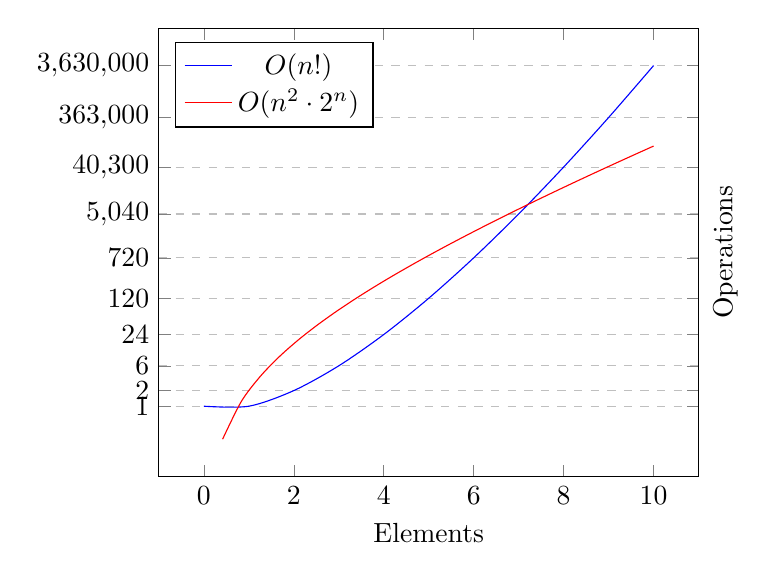
\begin{tikzpicture}
			\begin{semilogyaxis}[
					xlabel={Elements},
					ylabel={Operations},
					ylabel near ticks,
					ylabel style={at={(1.05,0.5)}, anchor=center},
					domain=0:10,
					ytick={0,1,2,6,24,120,720,5040,40320,362880,3628800},
					log ticks with fixed point,
					legend pos=north west,
					ymajorgrids=true,
					grid style=dashed,
				]
				\addplot+[mark=none,smooth] coordinates {
						(0,1) (1,1) (2,2) (3,6) (4,24) (5,120) (6,720) (7,5040)
						(8,40320) (9,362880) (10,3628800)
					};
				\addlegendentry{$O(n!)$}

				\addplot+[mark=none,smooth] expression {x^2 * 2^x};
				\addlegendentry{$O(n^2 \cdot 2^n)$}

			\end{semilogyaxis}
		\end{tikzpicture}
	\end{figure}
\end{center}

\begin{figure}[htbp]
	\centering
	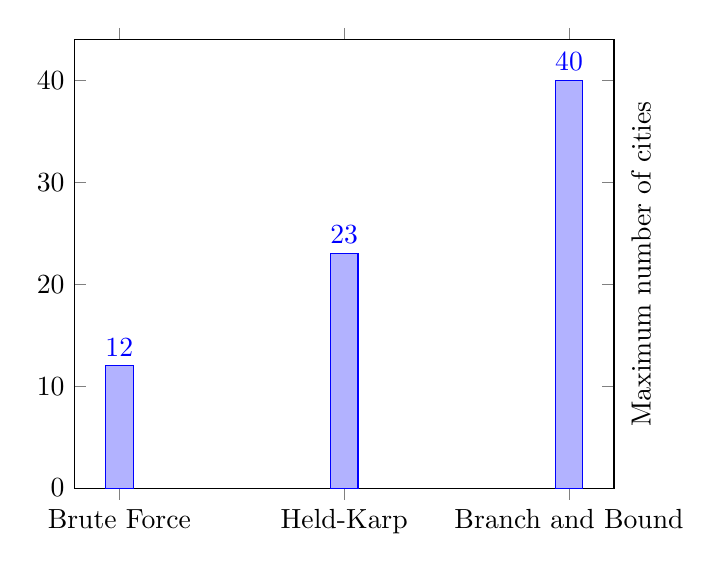
\begin{tikzpicture}
		\begin{axis}[
				ybar,
				ylabel={Maximum number of cities},
				symbolic x coords={Brute Force, Held-Karp, Branch and Bound},
				xtick=data,
				nodes near coords,
				nodes near coords align={vertical},
				ymin=0,
				ylabel near ticks,
				ylabel style={at={(1.05,0.5)}, anchor=center},
			]
			\addplot coordinates {(Brute Force,12) (Held-Karp,23) (Branch and Bound,40)};
		\end{axis}
	\end{tikzpicture}
	\caption{Maximum problem size solvable in one hour (approximate)}
	\label{fig:max-problem-size}
\end{figure}

\subsection{Advantages and Disadvantages}

In summary:

\textbf{Advantages:}
\begin{itemize}
	\item Guarantee of finding an optimal solution.
	\item Provide a benchmark for evaluating the performance of heuristic and metaheuristic algorithms.
\end{itemize}

\textbf{Disadvantages:}
\begin{itemize}
	\item Exponential time complexity that makes them impractical for large instances.
	\item Significant computational resources required even for moderate-sized problems.
	\item Dynamic programming and Held-Karp, while more efficient than the brute-force method, still face limitations due to their space complexity and the need for extensive computation.
\end{itemize}


\subsection{Concorde}


Concorde is considered one of the most efficient exact solvers for solving the \Gls{TSP}. Developed by a group of researchers led by Applegate et al., this solver exploits a combination of advanced methods such as branch-and-bound, cutting-plane, and linear and combinatorial programming techniques~\cite{Applegate2007}. Concorde is capable of solving \Gls{TSP} instances with thousands of cities in reasonable times, making it a reference tool for experimental comparisons and large-scale practical applications.

Concorde's efficiency is due to its ability to drastically reduce the search space through branch-and-bound, enhanced with the use of cutting planes to refine the lower bounds of solutions. In addition, Concorde implements effective heuristics to identify good initial solutions, which help limit the exploration of suboptimal solutions. Concorde has also been used to solve benchmark problems in the \Gls{TSP} literature, such as the TSPLIB problem instances \cite{TSPLIB}, demonstrating its effectiveness for real-world problem sizes~\cite{Cook2011}.

\textbf{Advantages:}
\begin{itemize}
    \item Ability to solve large \Gls{TSP} instances.
    \item Combined use of advanced optimization techniques.
    \item Efficient and well-documented implementations.
\end{itemize}

\textbf{Disadvantages:}
\begin{itemize}
    \item Requires high computational resources for extremely large instances.
    \item The complexity of the implemented techniques can make it difficult to adapt to problems slightly different from the \Gls{TSP}.
\end{itemize}


The exploration of exact algorithms lays the foundation for understanding the intrinsic computational complexities of the \Gls{TSP}. Although their practical application is limited by their computational demands, they remain crucial for theoretical analysis and for setting the stage for the alternative solution techniques discussed in subsequent chapters.

